\documentclass{article}
\usepackage{graphicx}
\usepackage{caption}
\usepackage{subcaption}
\usepackage{chngpage}

\begin{document}

\title{Estimating Ball-and-sticks Diffusion Model}
\author{Xinghua Zhu}

\maketitle

\section{Estimating single-fiber diffusivities}

A bunch of corpus callosum voxels are selected to determin diffusivities at single-fiber voxels.
The selected region is shown in Figure \ref{fig:cc}.
Totally 99 voxels within the selected region were used for diffusivity estimation.

The procedure of diffusivity estimation is as follows. First Schultz et al's algorithm \cite{Schultz2010} is applied to estimate the weight of the ball component. Then the Rician likelihood EM algorithm is used to estimate the ball-and-single-stick model with fixed weights. Those voxels with ball weights larger than 0.9 are regarded isotropic and abandoned. Among the remaining 51 voxels, histograms of the ball and stick diffusivities are plotted, as shown in Figure \ref{fig:diffusivities}.

In following experiments, the ball and stick diffusivites with highest density, namely $1.3\times 10^{-3}$ and $2.0\times 10^{-3}$, are used in estimations with fixed diffusivites. It should be noted that the ball and stick diffusivities are quite different from those estimated from the full tensor model, where typical diffusivities are $(1.2\times 10^{-3}, 0.4\times 10^{-3}, 0.4\times 10^{-3})$.

\begin{figure}[H]
  \centering
  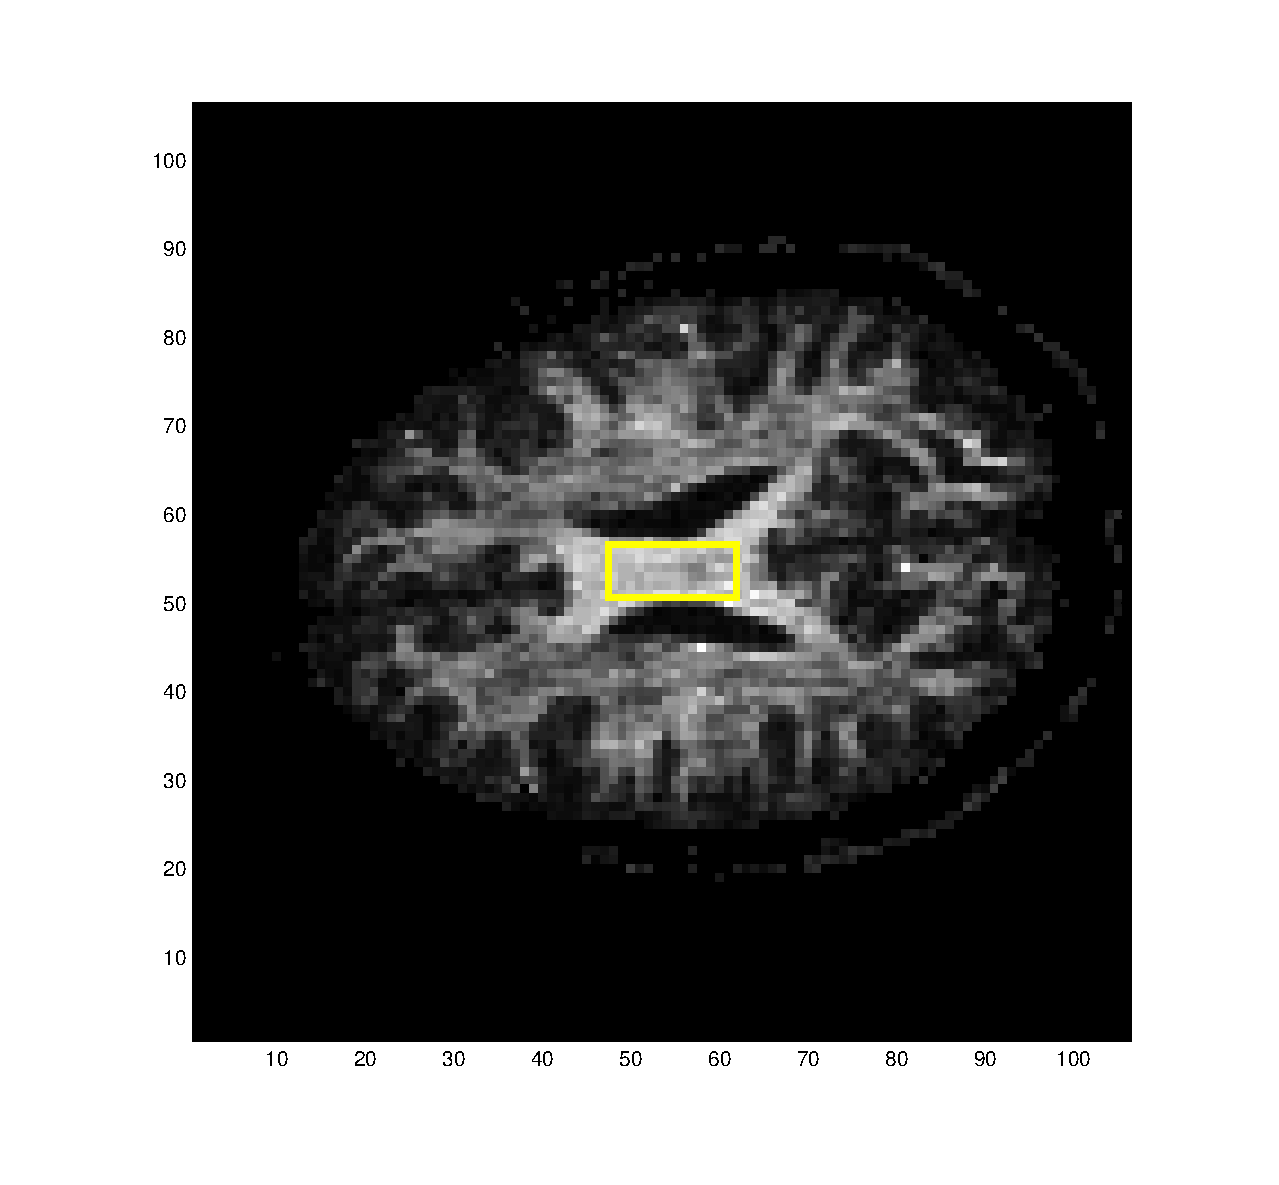
\includegraphics[width=\textwidth]{figures/corpus_callosum.eps}
  \caption{Voxels selected in corpus callosum for single-fiber diffusivity estimation (circled in yellow).}
  \label{fig:cc}
\end{figure}

\begin{figure}[H]
  \centering
  \begin{subfigure}{0.4\textwidth}
    \centering
    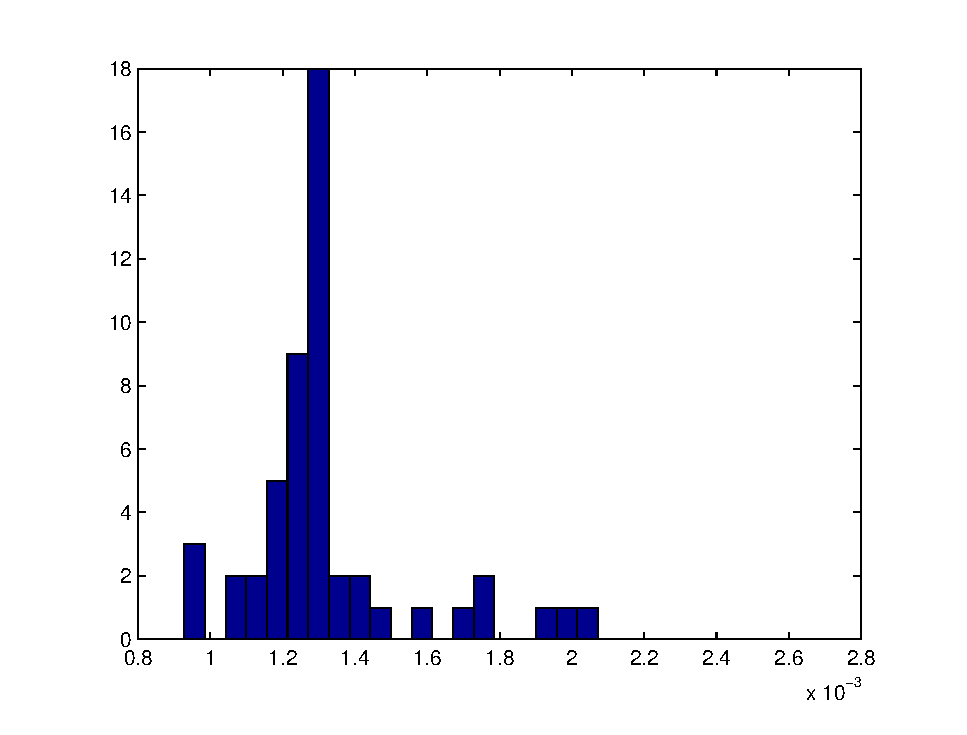
\includegraphics[width=\textwidth]{figures/cc_ball_diffus.eps}
    \caption{Ball diffusivity histogram}
  \end{subfigure}
  \begin{subfigure}{0.4\textwidth}
    \centering
    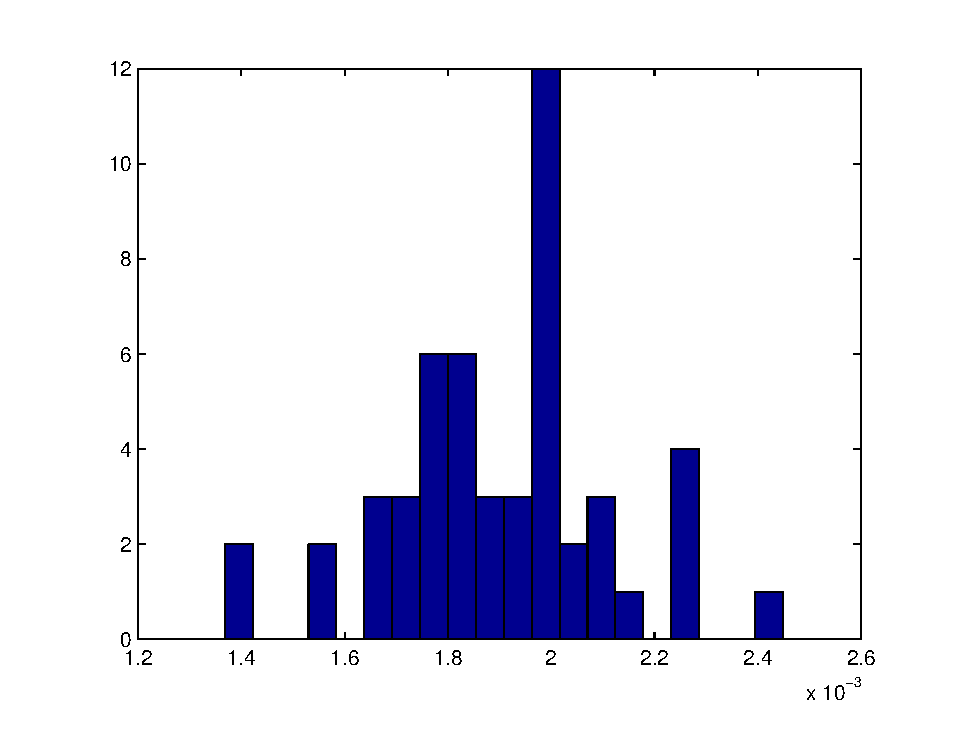
\includegraphics[width=\textwidth]{figures/cc_stick_diffus.eps}
    \caption{Sitck diffusivity histogram}
  \end{subfigure}
  \caption{Histogram of ball and stick diffusivities in the corpus callosum region.}
  \label{fig:diffusivities}
\end{figure}

\section{Coupling factor of the sparsity term}

Experiments are carried out on selected single- and crossing- fiber regions with different sparsity coupling factor. The selected voxels are shown in Figure \ref{fig:sparsity_roi}.

\begin{figure}[H]
  \centering
  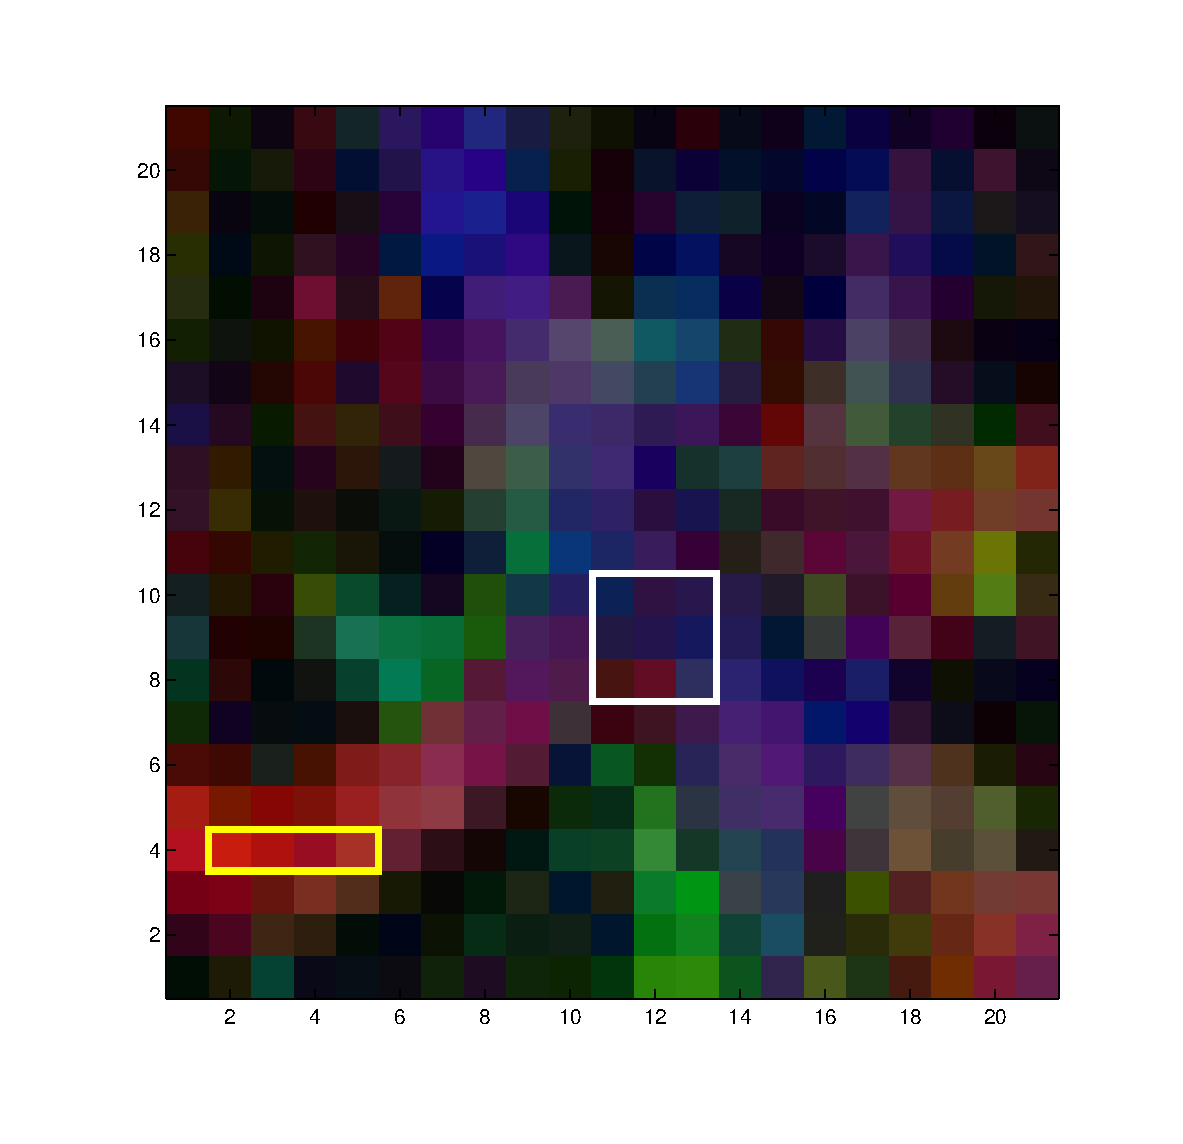
\includegraphics[width=\textwidth]{figures/sparsity_roi.eps}
  \caption{Single-fiber voxels (circled in yellow) and crossing-fiber voxels (circled in white) for sparsity coupling factor experiments.}
  \label{fig:sparsity_roi}
\end{figure}

For each of the selected voxel, a ball-and-3-sticks model was estimated. A full tensor model was first estimated to provide initial fiber directions. All weights are initalized equally (0.25 for each component). The ball and stick diffusivities are fixed at $1.3\times 10^{-3}$ and $2.0\times 10^{-3}$, resulted from the experiment described in Section 1.

In Figure \ref{fig:sparsity_plot}, the estimated component weights are plotted against the value of the coupling factor.

\begin{figure}[H]
  \begin{adjustwidth}{-\oddsidemargin}{-\rightmargin}
    \centering
    \begin{subfigure}{0.8\paperwidth}
      \centering
      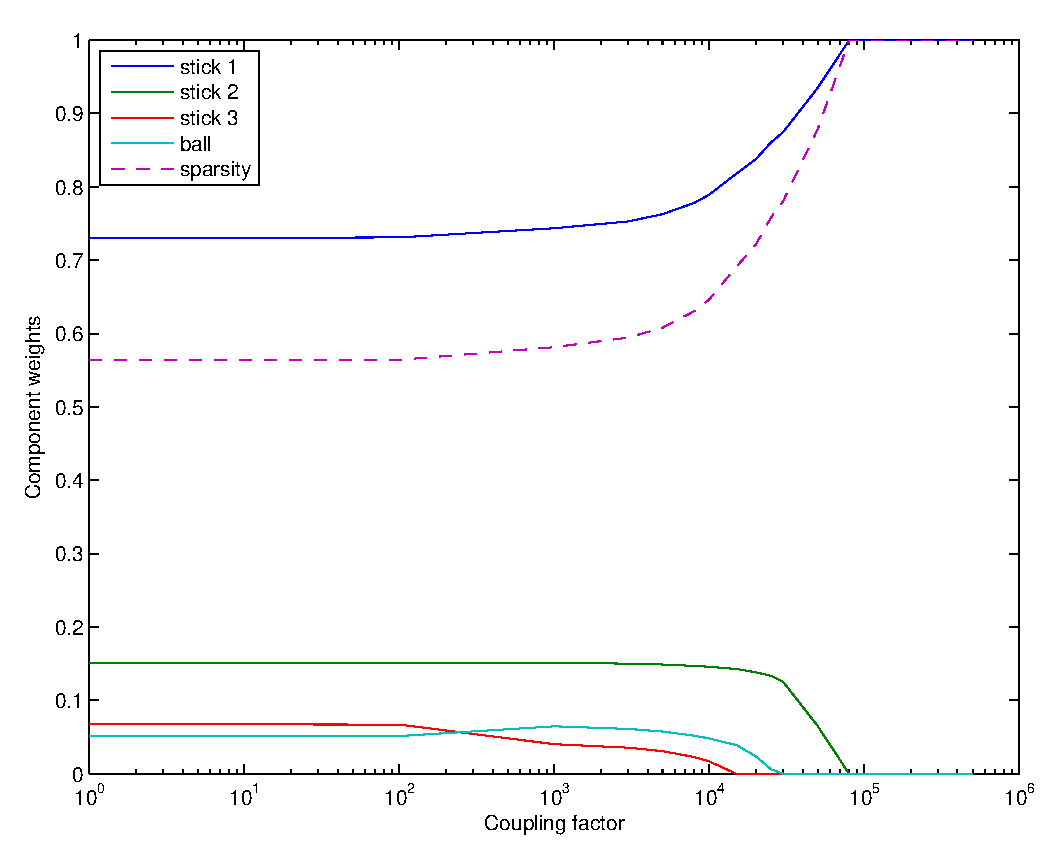
\includegraphics[width=0.3\textwidth]{figures/sparsity_50_43_single.eps} ~
      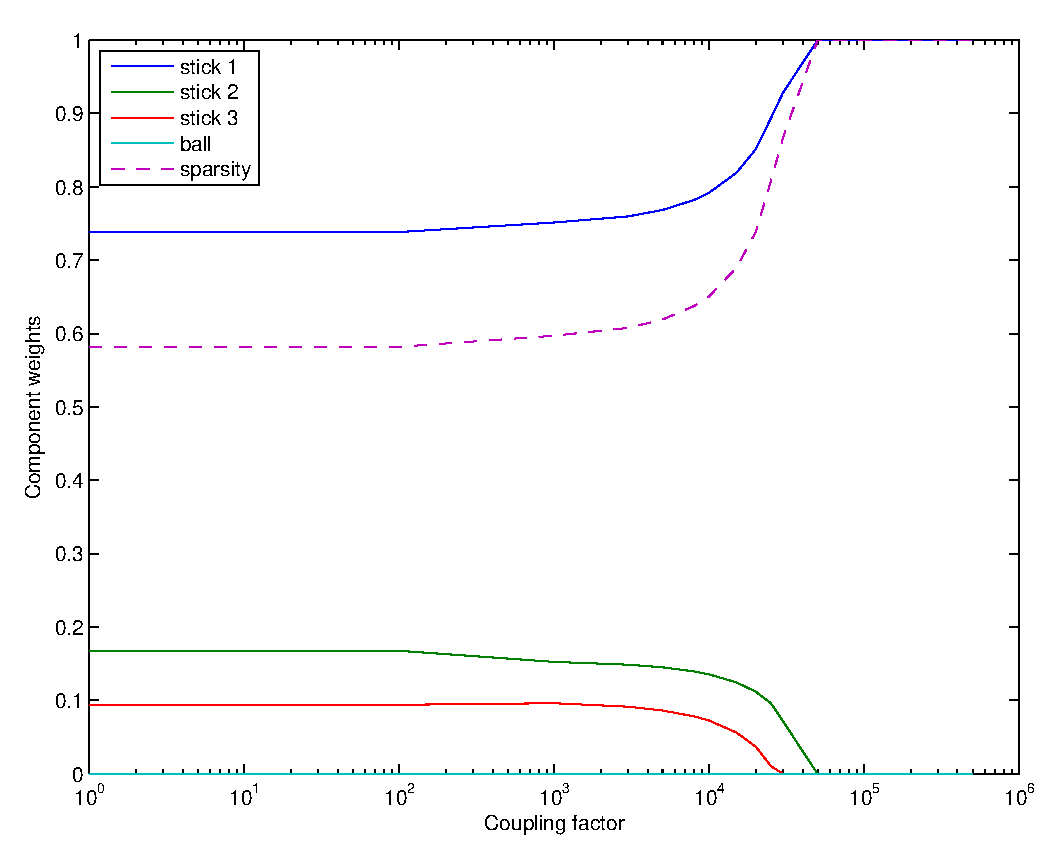
\includegraphics[width=0.3\textwidth]{figures/sparsity_51_43_single.eps} ~
      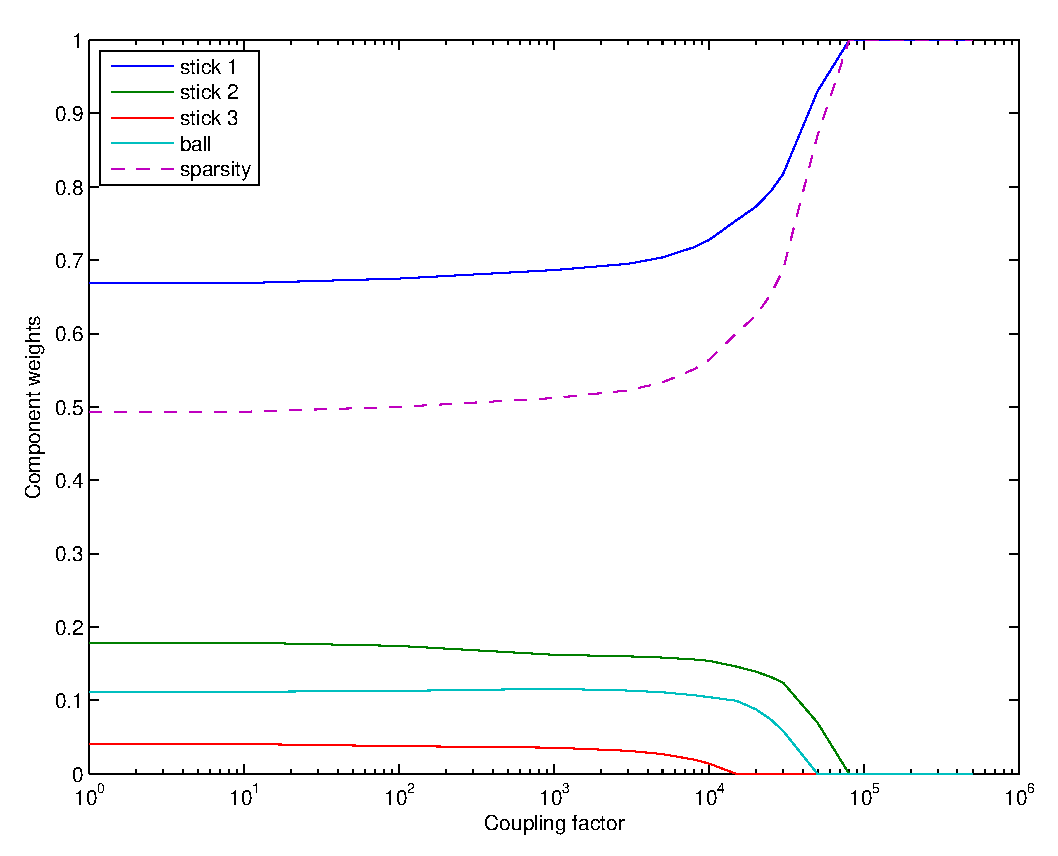
\includegraphics[width=0.3\textwidth]{figures/sparsity_52_43_single.eps}
      \caption{Single-fiber voxels}
    \end{subfigure}
    \begin{subfigure}{0.8\paperwidth}
      \centering
      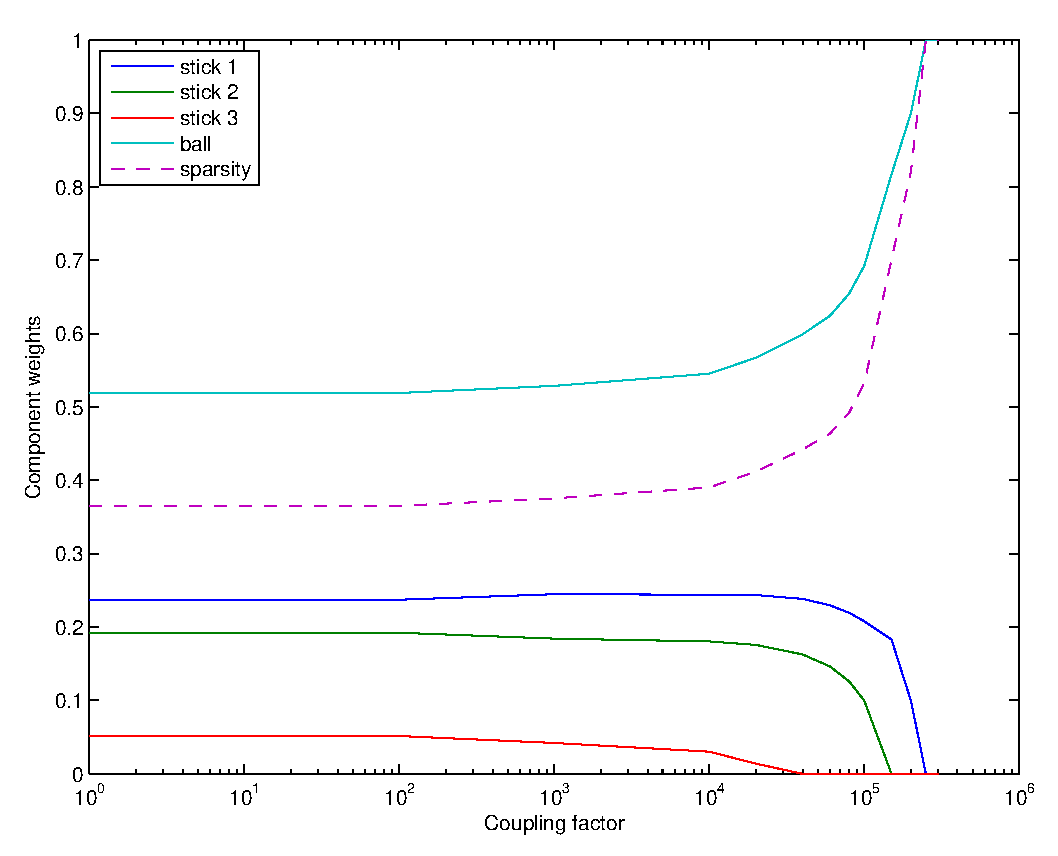
\includegraphics[width=0.3\textwidth]{figures/sparsity_60_47_cross.eps} ~
      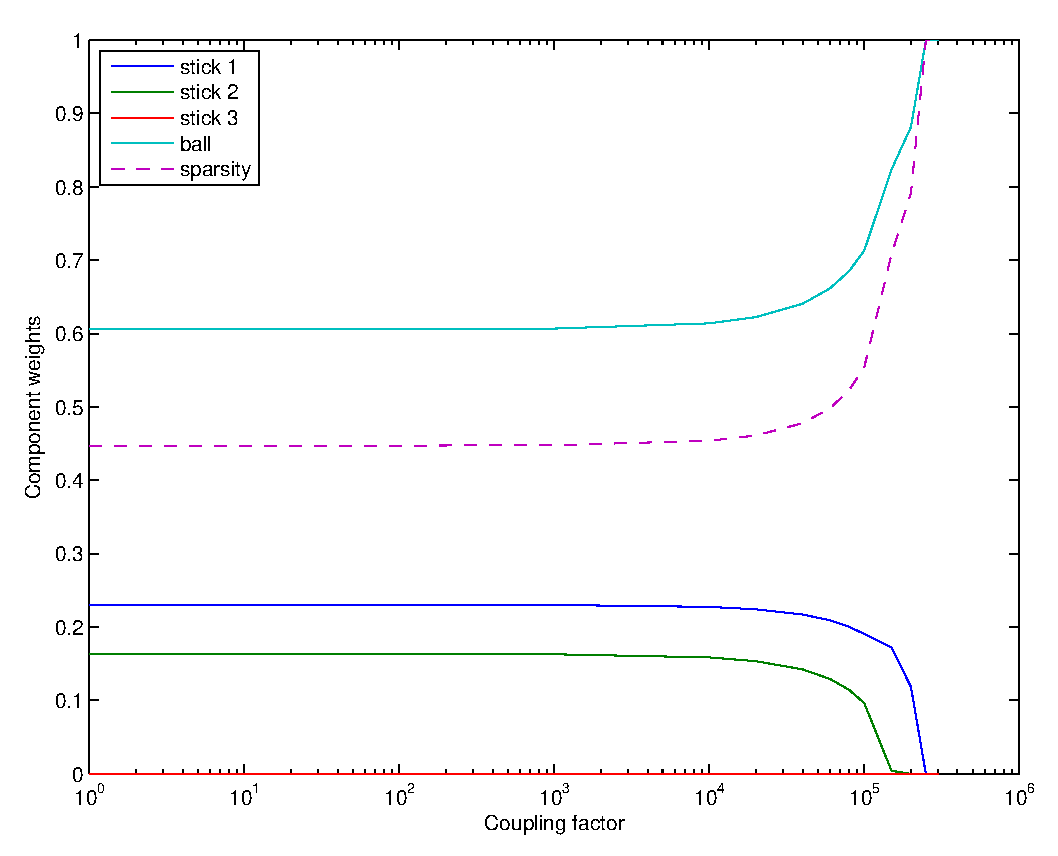
\includegraphics[width=0.3\textwidth]{figures/sparsity_60_48_cross.eps} ~
      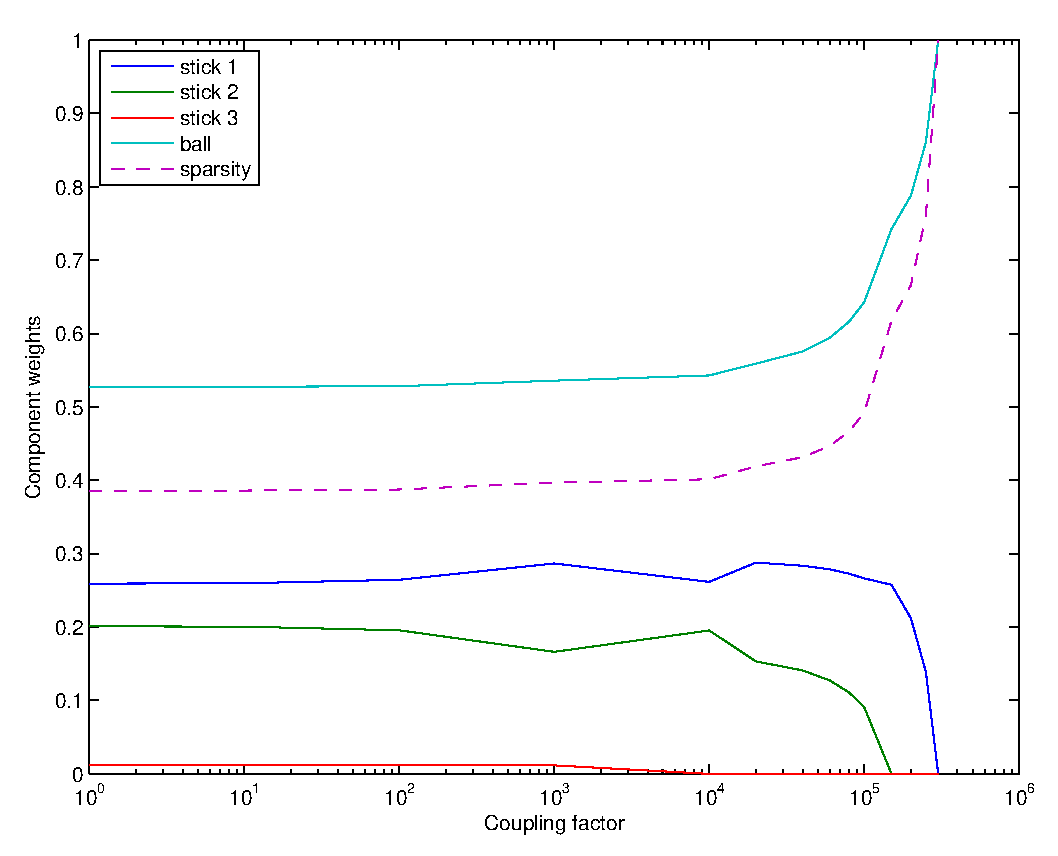
\includegraphics[width=0.3\textwidth]{figures/sparsity_60_49_cross.eps}    
      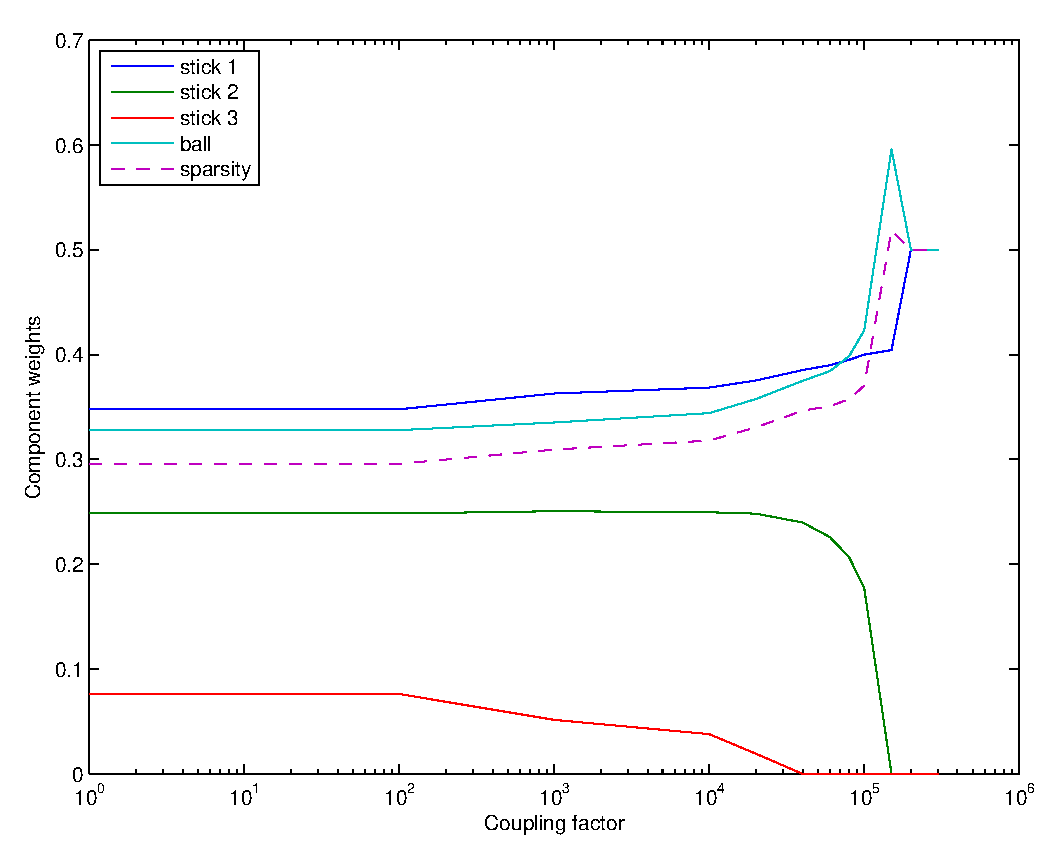
\includegraphics[width=0.3\textwidth]{figures/sparsity_61_47_cross.eps} ~
      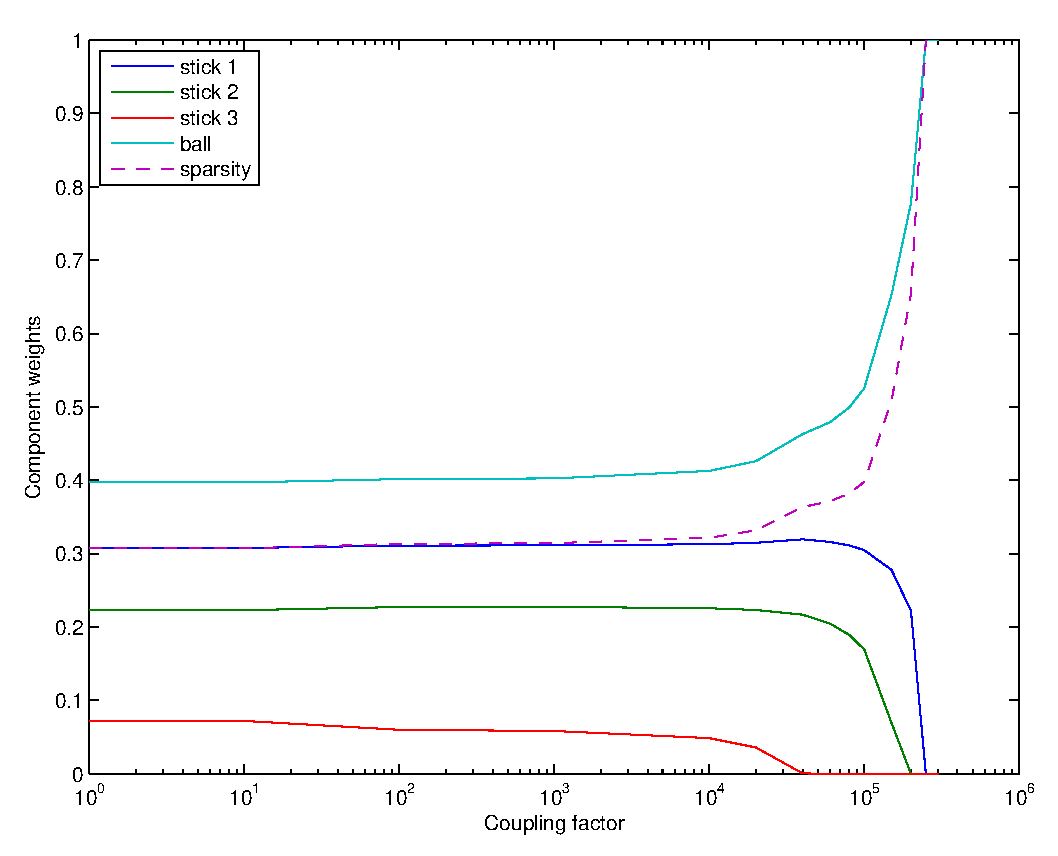
\includegraphics[width=0.3\textwidth]{figures/sparsity_61_48_cross.eps} ~
      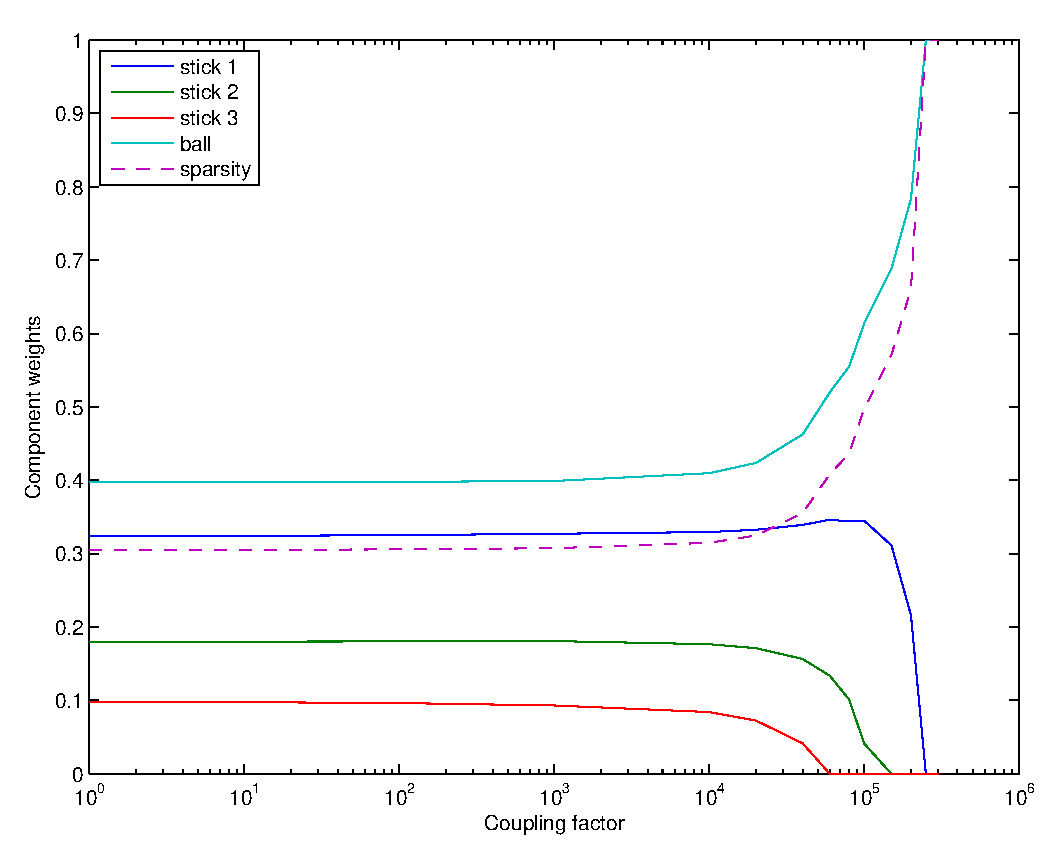
\includegraphics[width=0.3\textwidth]{figures/sparsity_61_49_cross.eps}    
      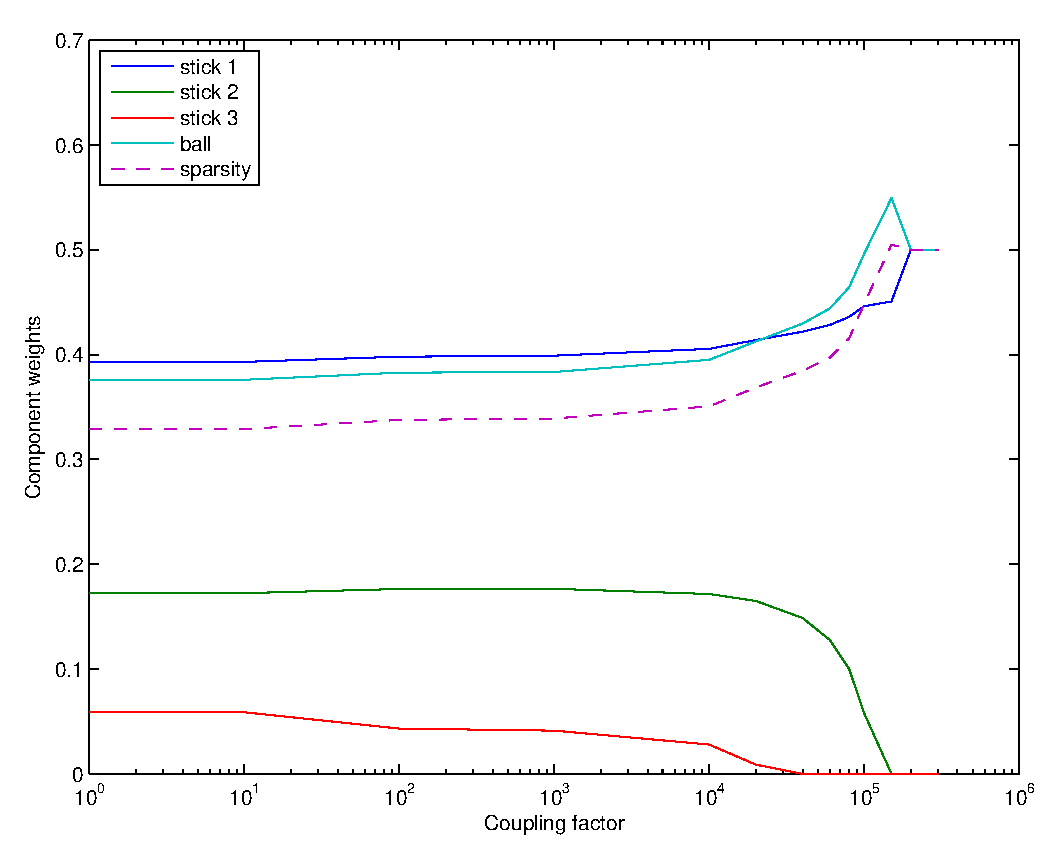
\includegraphics[width=0.3\textwidth]{figures/sparsity_62_47_cross.eps} ~
      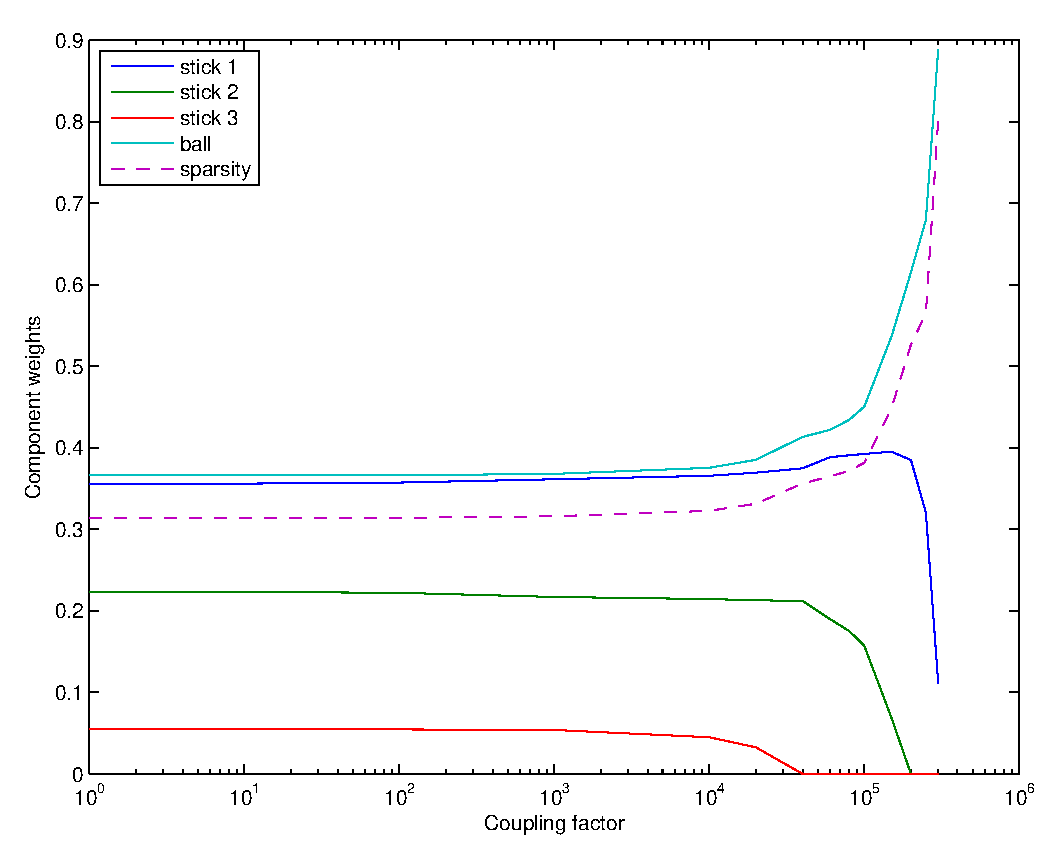
\includegraphics[width=0.3\textwidth]{figures/sparsity_62_48_cross.eps} ~
      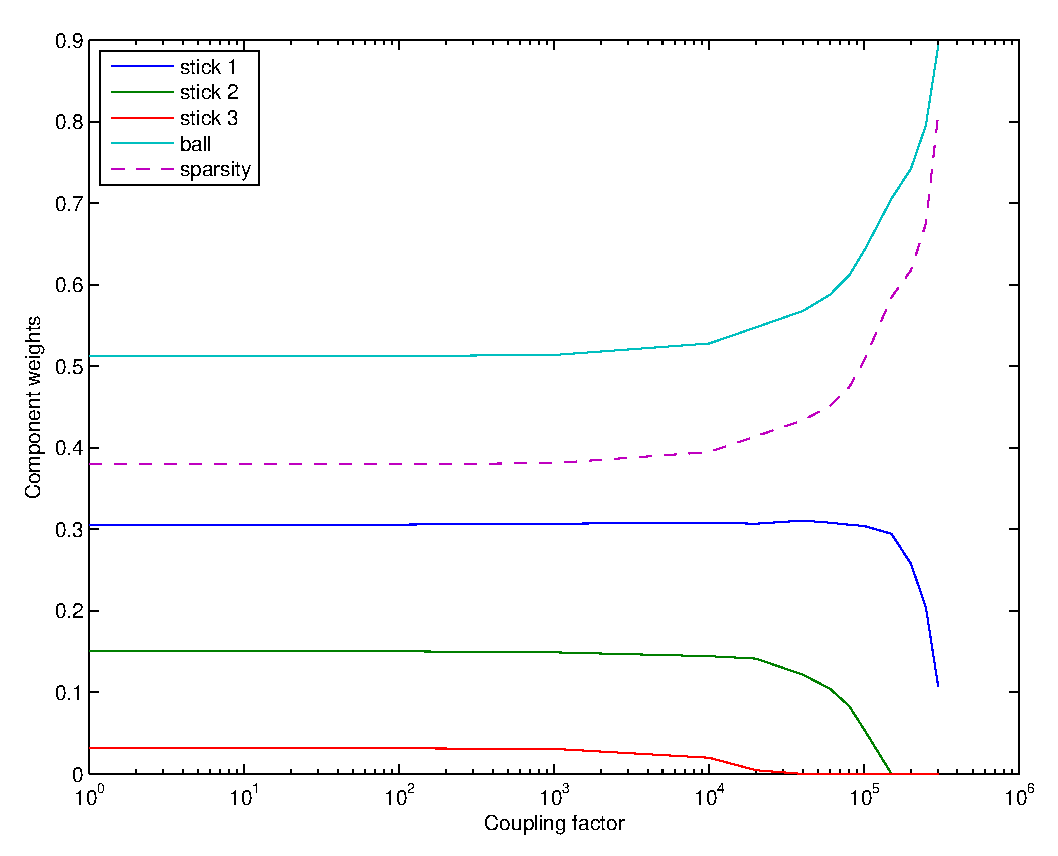
\includegraphics[width=0.3\textwidth]{figures/sparsity_62_49_cross.eps}  
      \caption{Crossing-fiber voxels}
    \end{subfigure}
  \end{adjustwidth}
  \caption{Estimated component weights against the sparsity coupling factor.}
  \label{fig:sparsity_plot}
\end{figure}

Figure \ref{fig:sparsity_plot} shows that the sparsity term pushes the redundant component to zero when the coupling factor reaches around $4\times 10^4$ at crossing-fiber voxels. At single-fiber voxels, the coupling factor must be increased to $1\times 10^5$ to eliminate all redundant components. Meanwhile, a moderate weight threshold for single-fiber voxels is $0.2$, while for crossing-fiber voxels it should be set at $0.1$.

\section{Regional results}

As a summary of the previous experiments, a ball-and-stick model estimation was performed on a region of interest with three coupling factors, namely 0, $4\times 10^4$ and $1\times 10^5$. Fiber directions are initialized with the three major axes of a full tensor fitted to the DW signal. The weights are initialized equally. Ball and stick diffusivities are fixed at $1.3\times 10^{-3}$ and $2.0\times 10^{-3}$.

Experimental results are shown in Figure \ref{fig:roi}. Components with weights less than 0.1 are not plotted in the figure. The lengths of the plotted directions are weighted by correspondent stick weight only.

\begin{figure}[H]
  \begin{adjustwidth}{-\oddsidemargin}{-\rightmargin}
  \centering
  \begin{subfigure}{0.3\paperwidth}
    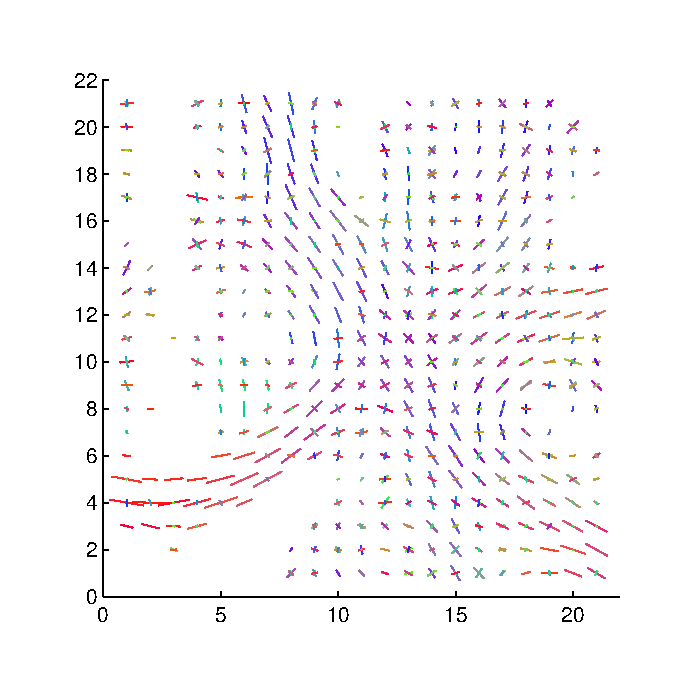
\includegraphics[width=\textwidth]{figures/brain_bas_s=0.eps}
    \caption{$\lambda=0$}
  \end{subfigure}
  ~
  \begin{subfigure}{0.3\paperwidth}
    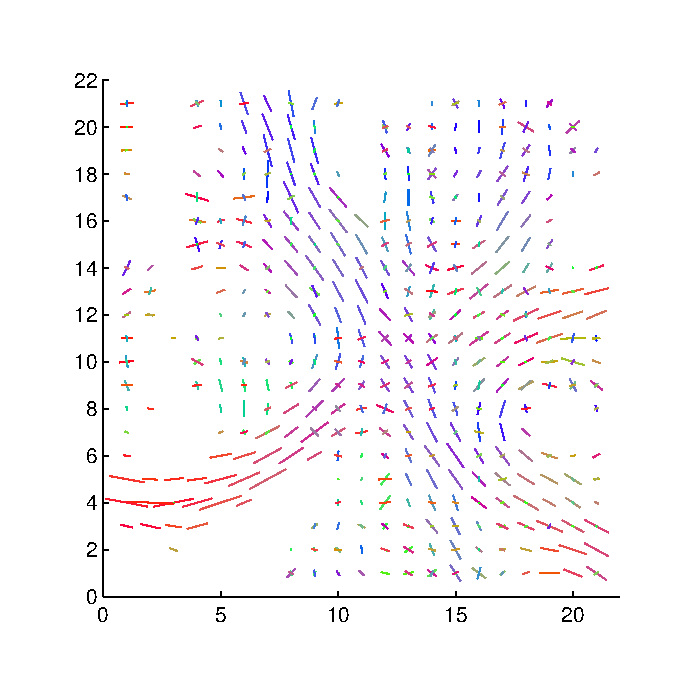
\includegraphics[width=\textwidth]{figures/brain_bas_s=4e4.eps}
    \caption{$\lambda=4\times 10^4$}
  \end{subfigure}
  ~
  \begin{subfigure}{0.3\paperwidth}
    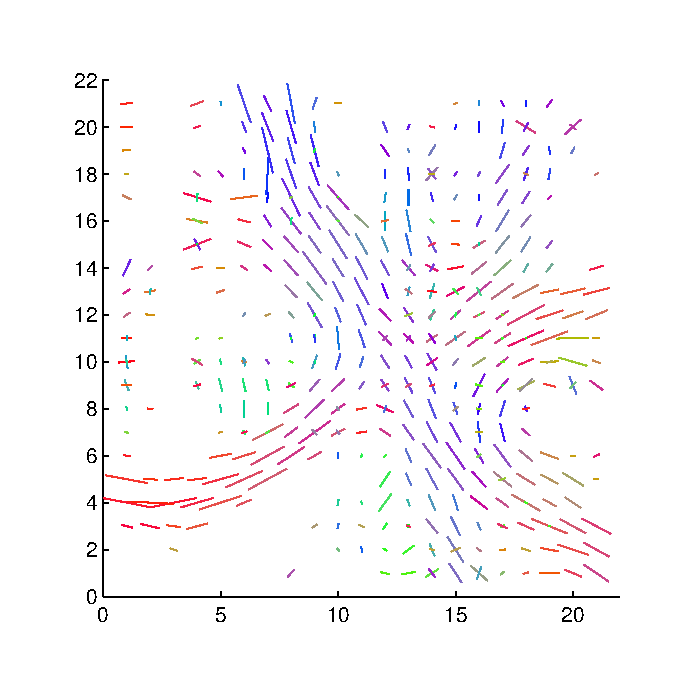
\includegraphics[width=\textwidth]{figures/brain_bas_s=1e5.eps}
    \caption{$\lambda=1\times 10^5$}
  \end{subfigure}
  \end{adjustwidth}
  \caption{Estimation result of real brain data with different coupling factor $\lambda$.}
  \label{fig:roi}
\end{figure}

\bibliographystyle{plain}
\bibliography{ref}

\end{document}